\chapter{The Polar Front as a major biogeographic boundary in the Southern Ocean} 
\label{ch:polarfront}

Sections of this chapter have been previously published in \bibentry{Wilkins:2012td}.

\section{Summary}

\section{Introduction}


\section{Methods}
\subsection{Sampling and metagenomic sequencing}

Sampling\footnote{Sampling was performed by Jeffrey M. Hoffman and Jeffrey B. Mcquaid} was conducted on board the RSV \emph{Aurora Australis} during cruise V3 CEAMARC/CASO (Collaborative East Antarctic Marine Census / Climate of Southern Ocean) from 13 December 2007 -- 26 January 2008. 
This cruise occupied the SR3 latitudinal transect from Hobart, Australia (44\textdegree S) to the Mertz Glacier, Antarctica (67\textdegree S) within a longitudinal range of 140--150\textdegree E.
Nineteen samples (16 surface, 3 deep) were obtained along almost the entire latitudinal range \figref{fig:samplemap}.

% the sample map
\begin{figure}[!ht]
  \centering
  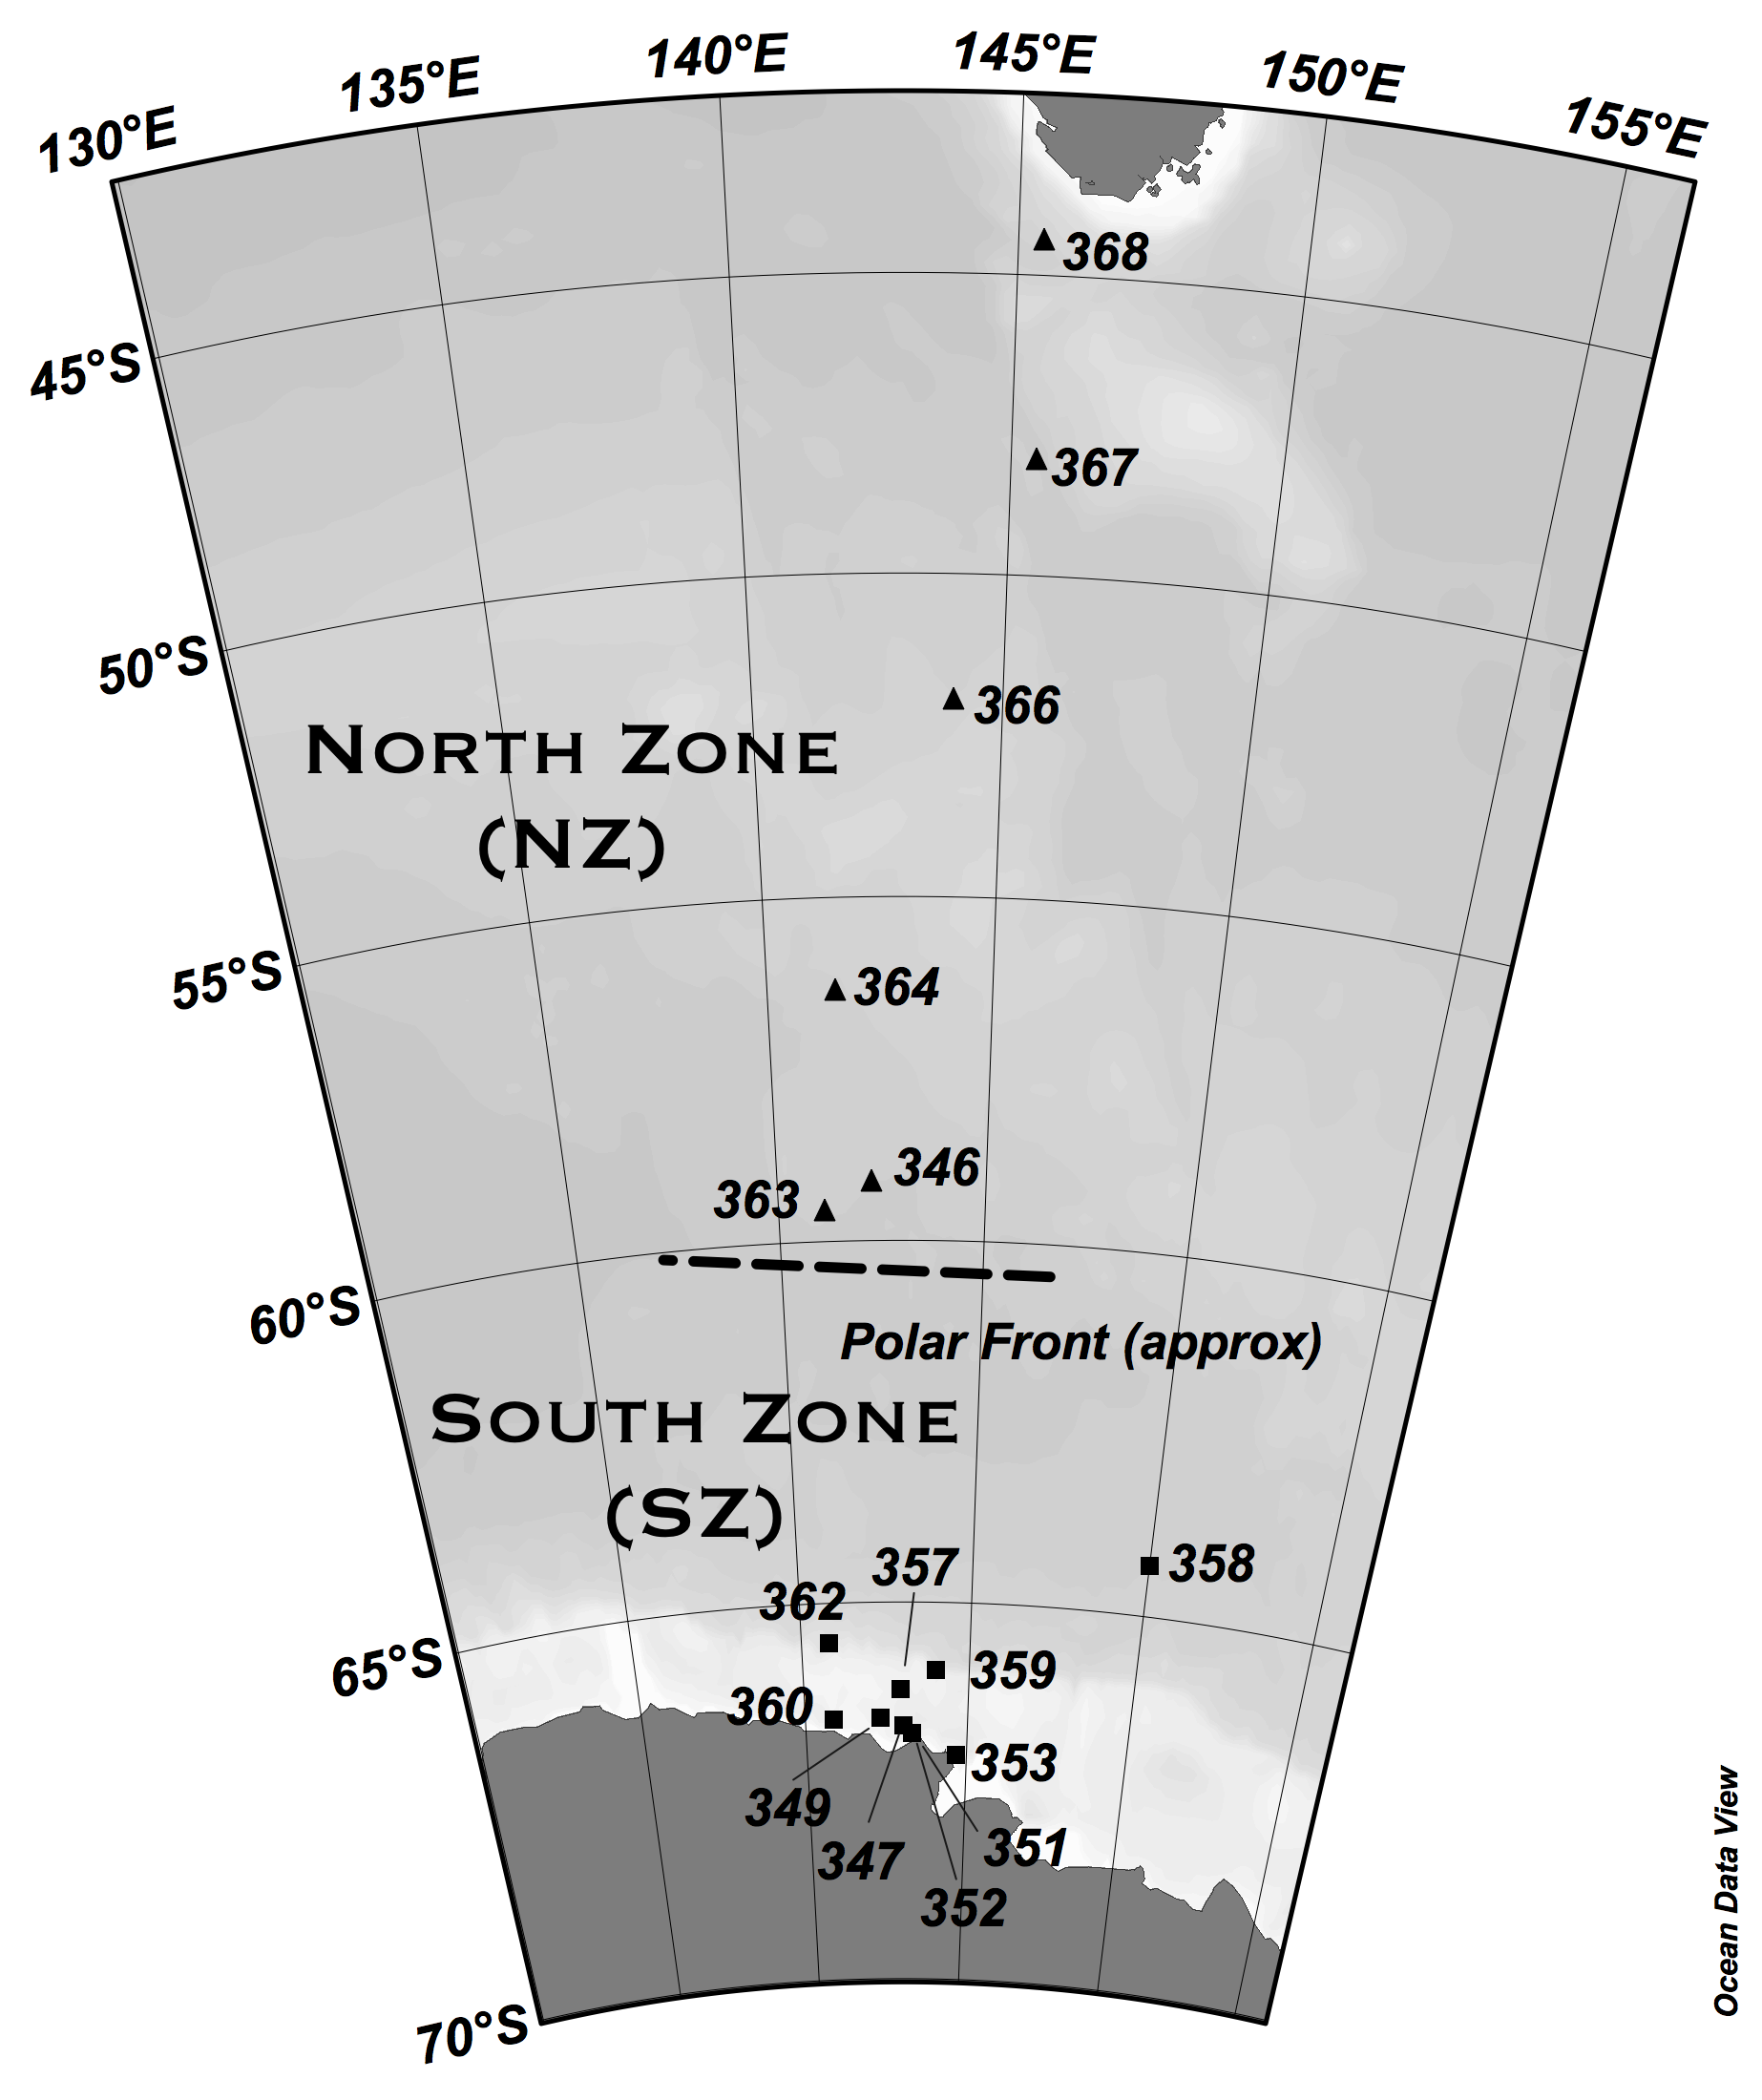
\includegraphics[width=\textwidth]{../polarfront/samplemap.png}
  \caption[Map showing sites of seawater samples used in the Polar Front study]{Sites of seawater samples used in this study. 
  Squares indicate surface samples from the North Zone; crosses samples from the South Zone. 
  The dashed line represents the Polar Front.}
  \label{fig:samplemap}
\end{figure}


A range of data were recorded by integrated instruments on the RSV \emph{Aurora Australis} including location, water column depth, water temperature, salinity, fluorescence and meterological data (TODO provide table).
These data were used to locate the (TODO abbreviations package? PFZ) based on a surface temperature gradient of $\sim$ 1.35 \textdegree{}C across a distance of 45--65 km, placing the (TODO abbreviations? PF) at approximately $-59.70$\textdegree of latitude, consistant with previous descriptions TODO EDITING HERE NEED SOKOLOV AND RINTOUL REF

\begin{sidewaystable}
\sffamily
\caption[Details of samples used in Polar Front study]{\sffamily{}Sampling time, location and physicochemical properties of samples used in this study.
All data were retrieved from underway instruments aboard the RSV \textit{Aurora Australis}.}
\label{tab:samplelist}
\smallskip
\begin{tabularx}{\textheight}{lllXXXXXXXX}
\toprule
\textbf{Sample} & \textbf{Zone} & \textbf{Date} & \textbf{Latitude} & \textbf{Longitude} & \textbf{Water \linebreak Column \linebreak Depth (m)} & \textbf{Sample Depth (m)} & \textbf{Temperature (\textdegree{}C)} & \textbf{Salinity (PSU)} & \textbf{Fluorescence \linebreak (\textmu{}gL\textsuperscript{\textminus{}1})} & \textbf{Volume \linebreak filtered (L)}\\
\midrule

346 & North & 20/12/2007 & \textminus{}59.31 & 142.59 & 4294 & 2 & 2.9 & 33.75 & 0.3 & 500\\
347 & South & 23/12/2007 & \textminus{}66.02 & 142.74 & 450 & 2 & 0.6 & 34.20 & 4.0 & 250\\
349 & South & 27/12/2007 & \textminus{}66.57 & 142.32 & 370 & 1.5 & \textminus{}1.3 & 34.40 & 2.3 & 250\\
351 & South & 28/12/2007 & \textminus{}66.56 & 143.43 & 823 & 1.5 & \textminus{}0.6 & 34.30 & 1.3 & 500\\
352 & South & 29/12/2007 & \textminus{}66.77 & 143.32 & 164 & 2.5 & \textminus{}0.8 & 34.30 & 3.1 & 500\\
353 & South & 30/12/2007 & \textminus{}67.05 & 144.68 & 180 & 2 & \textminus{}1.8 & 34.40 & 0.3 & 500\\
357 & South & 05/01/2008 & \textminus{}66.17 & 143.02 & 580 & 2 & \textminus{}0.4 & 34.15 & 2.5 & 500\\
358 & South & 09/01/2008 & \textminus{}64.30 & 150.03 & 3550 & 2 & 0 & 33.55 & 0.5 & 500\\
359 & South & 12/01/2008 & \textminus{}66.19 & 143.53 & 540 & 2 & \textminus{}0.2 & 34.21 & 2.5 & 500\\
360 & South & 13/01/2008 & \textminus{}66.58 & 141.02 & 316 & 2 & \textminus{}0.7 & 34.04 & 6.2 & 500\\
362 & South & 19/01/2008 & \textminus{}65.54 & 140.83 & 1064 & 2 & 0.7 & 32.20 & 0.5 & 500\\
363 & North & 22/01/2008 & \textminus{}60.00 & 141.31 & 4473 & 2 & 3.3 & 33.77 & 0.1 & 500\\
364 & North & 23/01/2008 & \textminus{}56.70 & 141.88 & 3693 & 2 & 4 & 33.70 & 0.5 & 500\\
366 & North & 24/01/2008 & \textminus{}52.02 & 144.14 & 3180 & 2 & 7.6 & 33.84 & 0.3 & 500\\
367 & North & 25/01/2008 & \textminus{}48.25 & 145.90 & 3490 & 2 & 11 & 34.43 & 0.2 & 500\\
368 & North & 26/01/2008 & \textminus{}44.72 & 145.78 & 3201 & 2 & 14.8 & 34.96 & 1.3 & 560\\

\bottomrule
\end{tabularx}
\end{sidewaystable}


At each station, $\sim$ 250--560 L of seawater was pumped from $\sim$ 1.5--2.5 m below the sea surface into drums stored at ambient temperature on deck. 
In the case of deep samples, $\sim$ 225--230 L of seawater was collected opportunistically from Niskin bottles attached to a CTD (Conductivity, Temperature and Depth TODO give infor on CTD - SeaBird?) instument operated by an unrelated oceanographic project.
Seawater samples were prefiltered through a 20 \textmu{}m plankton net, then filtrate was captured on sequential 3.0 \textmu{}m, 0.8 \textmu{}m and 0.1 \textmu{}m polyethersulfone membrane filters (Supor membrane disc filter; Pall Life Sciences TODO location), and immediately stored at $-20$ $^\circ$C \cite{Rusch:2007ez,Ng:2010cd}.

DNA extraction\footnote{DNA extraction was performed by Cynthia Andrews-Pfannkoch and others at the J. Craig Venter Institute} was performed at the J. Craig Venter Institute (Rockville, USA) as described in \citet{Rusch:2007ez}.
Pyrosequencing was performed on a GS20 FLX Titanium instrument (Roche, Branford, USA) also at the J. Craig Venter Institute as described in \citet{Lauro:2010jna}.
Duplicate reads and reads with many pyrosequencing errors were removed as described in \citet{Lauro:2010jna}.

\subsection{Phylogenetic analysis of metagenomic data}
\subsection{Functional analysis of metagenomic data}

\section{Results}
\subsection{Metagenomic sequencing}
\subsection{Phylogenetic analysis of metagenomic data}
\subsection{Functional analysis of metagenomic data}

\section{Discussion}

\section{Conclusions}

